\documentclass{article}
\usepackage{../csci-246-fall2018/hw/template/fasy-hw}
\usepackage{amsmath}
\usepackage{cancel}
\usepackage{hyperref}

\author{Nathan Stouffer}
\problem{10-1}
% \problem{A-B} means Problem Set A, Problem B.
\collab{none}
% or give names, e.g., \collab{Alyssa P. Hacker and A. Student}

\begin{document}

\section*{50 Free Points}

\problem{10-2}
\collab{Kevin Browder}
\clearpage
\header

\begin{enumerate}[2.1]
	\item For this weighted coin, P(Heads)=0.75 and P(Tails)=0.25, therefore $P(\text{0 Heads})= \binom{3}{0}*\dfrac{3}{4}^0*\dfrac{1}{4}^3= \dfrac{1}{64}$, $P(\text{1 Head})= \binom{3}{1}*\dfrac{3}{4}^1*\dfrac{1}{4}^2= \dfrac{9}{64}$, $P(\text{2 Heads})= \binom{3}{2}*\dfrac{3}{4}^2*\dfrac{1}{4}^1= \dfrac{27}{64}$, $P(\text{3 Heads})= \binom{3}{3}*\dfrac{3}{4}^3*\dfrac{1}{4}^0= \dfrac{27}{64}$
	\begin{center}
		\begin{tabular}{ |c|c|c|c|c| } 
			\hline
			X = number of heads & 0 & 1 & 2 & 3 \\ 
			P(X) & $\dfrac{1}{64}$ & $\dfrac{9}{64}$ & $\dfrac{27}{64}$ & $\dfrac{27}{64}$ \\ 
			\hline
		\end{tabular}
	\end{center}
	$E(X)=0*\dfrac{1}{64} + 1*\dfrac{9}{64} + 2*\dfrac{27}{64} + 3*\dfrac{27}{64}=\dfrac{9}{4}$ \\
	$V(X)= E(X^2) - E(X)^2 = (0^2*\dfrac{1}{64} + 1^2*\dfrac{9}{64} + 2^2*\dfrac{27}{64} + 3^2*\dfrac{27}{64}) - \dfrac{9}{4}^2 = \dfrac{9}{16}$
	\item Multiplying the results of rolling two dice
		\graphicspath{ {possibility_tree} }
		\begin{figure}[h]
			\centering
			\fbox{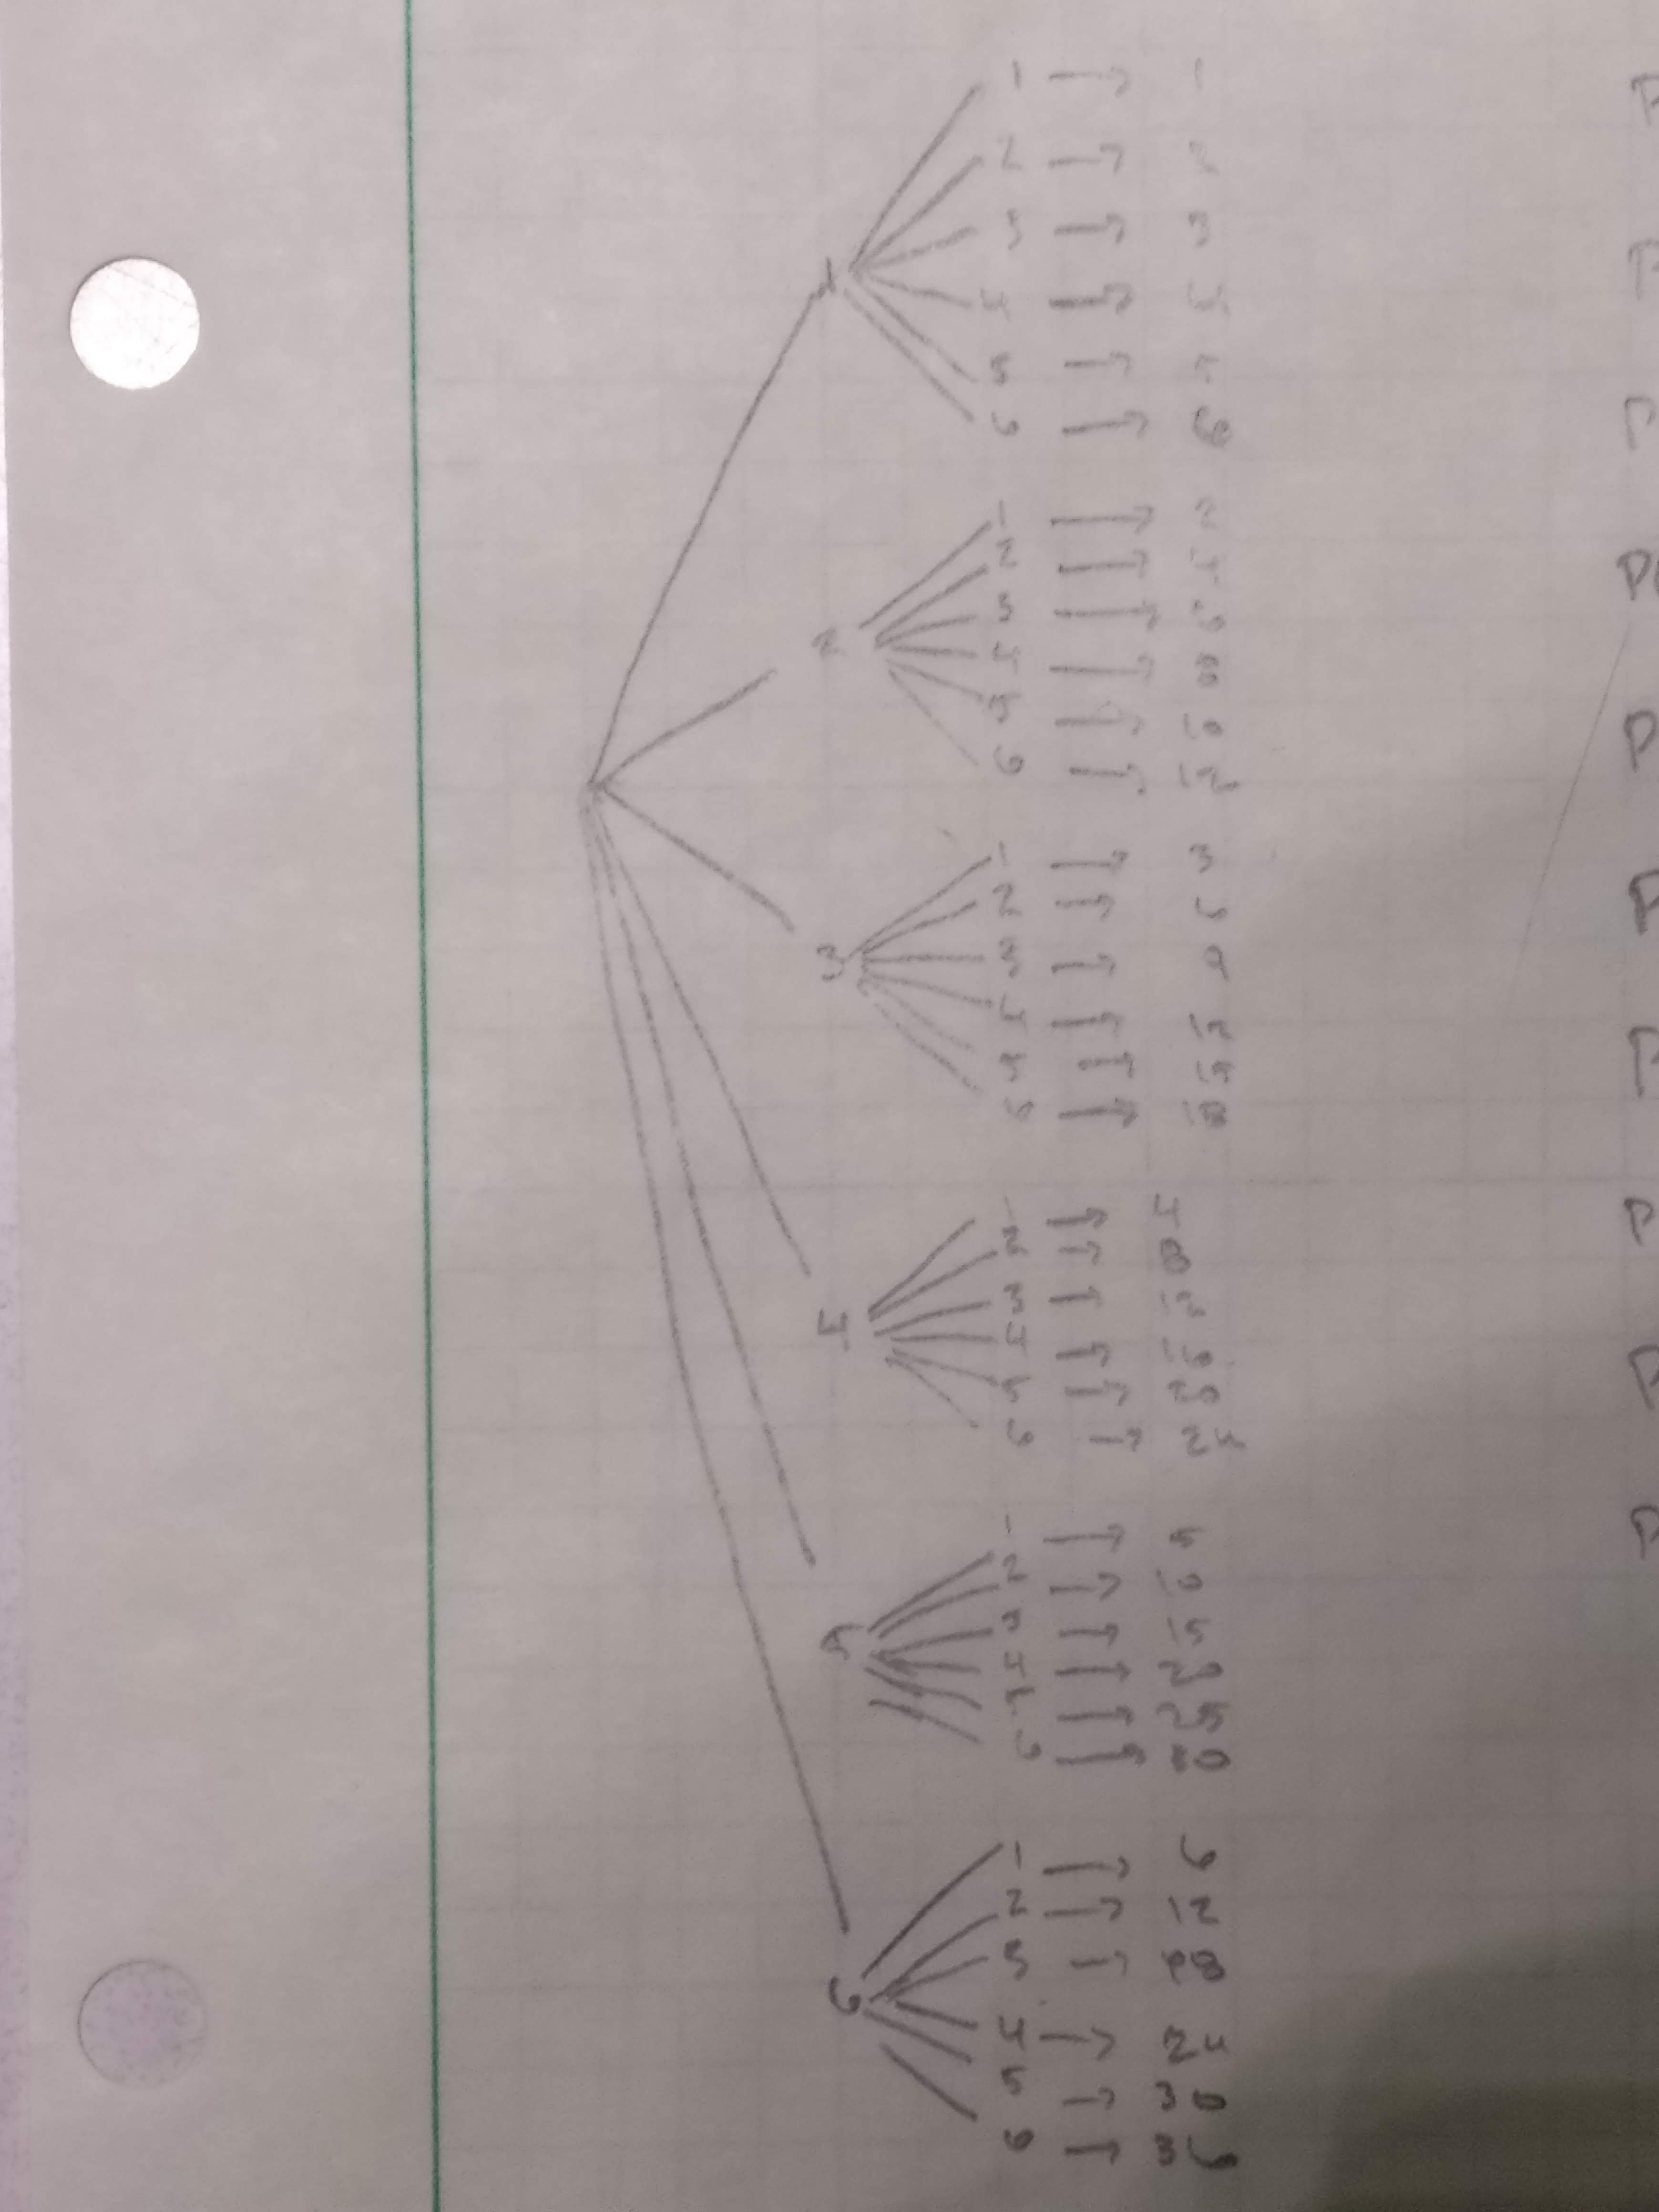
\includegraphics[width=5cm]{possibility_tree}}
			\caption{Possibility tree for rolling two dice}
		\end{figure}
		\begin{center}
			\begin{tabular}{ |c|c|c|c|c|c|c|c|c|c|c|c|c|c|c|c|c|c|c| } 
				\hline
				X = product & 1 & 2 & 3 & 4 & 5 & 6 & 8 & 9 & 10 & 12 & 15 & 16 & 18 & 20 & 24 & 25 & 30 & 36 \\ 
				P(X) & $\dfrac{1}{36}$ & $\dfrac{1}{18}$ & $\dfrac{1}{18}$ & $\dfrac{1}{12}$ & $\dfrac{1}{18}$ & $\dfrac{1}{9}$ & $\dfrac{1}{18}$ & $\dfrac{1}{36}$ & $\dfrac{1}{18}$ & $\dfrac{1}{9}$ & $\dfrac{1}{18}$ & $\dfrac{1}{36}$ & $\dfrac{1}{18}$ & $\dfrac{1}{18}$ & $\dfrac{1}{18}$ & $\dfrac{1}{36}$ & $\dfrac{1}{18}$ & $\dfrac{1}{36}$ \\ 
				\hline
			\end{tabular}
		\end{center}
		$E(X) = 1*\dfrac{1}{36} + 2*\dfrac{1}{18} + 3*\dfrac{1}{18} + 4*\dfrac{1}{12} + 5*\dfrac{1}{18} + 6*\dfrac{1}{9} + 8*\dfrac{1}{18} + 9*\dfrac{1}{36} + 10*\dfrac{1}{18} + 12*\dfrac{1}{9} + 15*\dfrac{1}{18} + 16*\dfrac{1}{36} + 18*\dfrac{1}{18} + 20*\dfrac{1}{18} + 24*\dfrac{1}{18} + 25*\dfrac{1}{36} + 30*\dfrac{1}{18} + 36*\dfrac{1}{36} = 12.25$ \\
		$V(X) = E(X^2) - E(X)^2 = (1^2*\dfrac{1}{36} + 2^2*\dfrac{1}{18} + 3^2*\dfrac{1}{18} + 4^2*\dfrac{1}{12} + 5^2*\dfrac{1}{18} + 6^2*\dfrac{1}{9} + 8^2*\dfrac{1}{18} + 9^2*\dfrac{1}{36} + 10^2*\dfrac{1}{18} + 12^2*\dfrac{1}{9} + 15^2*\dfrac{1}{18} + 16^2*\dfrac{1}{36} + 18^2*\dfrac{1}{18} + 20^2*\dfrac{1}{18} + 24^2*\dfrac{1}{18} + 25^2*\dfrac{1}{36} + 30^2*\dfrac{1}{18} + 36^2*\dfrac{1}{36}) - (12.25)^2 = 79.965$
\end{enumerate}

\problem{10-3}
\collab{none}
\clearpage
\header

The limitation of drawing only infinite straight lines to create maps makes all such maps two-color maps in the plane. This is because each edge extends beyond the face to infinity. If each edge extends beyond the face it creates, then no more than two adjacent faces (excluding vertexes) can be drawn. Therefore, all maps in the plane drawn only with infinite straight lines can be colored with two colors. 

\problem{10-4}
\collab{Kevin Browder}
\clearpage
\header

\begin{enumerate}[4.1]
	\item 	Problem: $T(n) = 2T(n/4) +\log(n)$\\
		If $\exists \epsilon > 0$ such that $f(n) = O(n^{\log_ba-\epsilon})$, then $T(n)$ is $\Theta(n^{\log_ba})$. In this case, $a = 2, b = 4, c = 0, n_0 = 1, f(n) = \log(n)$ if $\epsilon = 1/4$ then $n^{\log_ba-\epsilon} = n^{\log_24-\frac{1}{4}} = n^{\frac{1}{4}}$ and $f(x)$ is $O(n^\frac{1}{4})$ so case 1 is true for $T(n)$ which means that $T(n) = \Theta(n^{\log_ba})$. Therefore, $T(n)$ is $\Theta(n^{log_24}) = \Theta(n^\frac{1}{2})$ 
	\item Problem: $T(n) = 5T(\dfrac{n}{5}) + \dfrac{n}{3}$\\
		$F(n) = \dfrac{n}{3}$ and $n^{\log_ba} = n^{\log_55} = n$\\
		$F(n) = \Theta(n)$ because they have the same power (one). This means that Case 2 of Master's Theorem will be used.From here we use the definition of $\Theta$: $\dfrac{1}{c}*n \leq \dfrac{n}{3} \leq c*n$ where $c, n \in \mathbb{R}$. We can then choose $c = 3$ to make this expression true for $n_0 = 1$: $\dfrac{1}{3}*1 \leq \dfrac{1}{3} \leq 3*1$, which is true.
\end{enumerate}

\problem{10-5}
\collab{none}
\clearpage
\header

\section*{Importance of Master's Theorem}

The Master's Theorem is important in Computer Science because it provides an easy way for recurrence relations to be represented as a time complexity. The three cases cover all relations of the form $T(n)=a*T(\dfrac{n}{b}) + f(n)$ and give mathematicians and computer scientists a shortcut when looking at the efficiency of algorithms. This allows for problems to computed much quicker and with less error because there exists a standard formula that can be used as a "plug and chug" method.

\end{document}

